%
%  Peter Vermeer
%
\documentclass[12pt,fullpage]{article}
\usepackage{fullpage}
\usepackage{psfrag}                                          % LaTeX graphics tool
\usepackage{pslatex}                                         % avoids the default cmr font
\usepackage{graphicx}                                        % graphics package 
\usepackage{epsfig}                                          % figures
\usepackage{hyperref}
\usepackage{color}

\begin{document}

\noindent
{\bf Standard Cauchy distribution}  (from \color{blue}\url{http://www.math.wm.edu/~leemis/chart/UDR/UDR.html}\color{black})

\noindent
The shorthand $X \sim {\rm Cauchy}(1,0)$ is used to indicate that the
random variable $X$ has the standard Cauchy distribution.
A standard Cauchy random variable $X$ has probability density function 
$$
f(x) = {\frac {1}{\pi \, \left( 1+{x}^{2} \right) }} \qquad \qquad -\infty<x<\infty.
$$
The probability density function is illustrated below.
{\begin{figure}[h!]
\begin{center}
\psfrag{labx}{$x$}
\psfrag{labf}{$f(x)$}
\includegraphics[width=3.2in]{StandardcauchyPlot.ps}
\end{center}
\end{figure}}\\
The cumulative distribution function on the support of $X$ is
$$
F(x) = P(X \le x) = {\frac {\pi +2\,\arctan \left( x \right) }{2\pi }} \qquad \qquad -\infty<x<\infty.
$$
The survivor function on the support of $X$ is
$$
S(x) = P(X \ge x) = {\frac {\pi -2\,\arctan \left( x \right) }{2\pi }} \qquad \qquad -\infty<x<\infty.
$$
The hazard function on the support of $X$ is
$$
h(x) = \frac{f(x)}{S(x)} = {\frac {2}{ \left( 1+{x}^{\kern 0.08 em 2} \right)  \left( \pi -2\,\arctan \left( x \right)  \right) }} \qquad \qquad -\infty<x<\infty.
$$
The cumulative hazard function on the support of $X$ is
$$
H(x) = - \ln S(x) = \ln  \left( 2 \right) +\ln  \left( \pi  \right) -\ln  \left( \pi -2\,\arctan \left( x \right)  \right)   \qquad \qquad -\infty<x<\infty.
$$
The inverse distribution function of $X$ is
$$
F ^ {-1}(u) = -\cot(u\cdot \pi) \qquad \qquad 0 < u < 1.
$$
The median of $X$ is 0.
$$
$$
The moments of $X$ are undefined. It follows that the population mean, variance, skewness, and kurtosis of $X$ are also undefined.

\vspace{0.1in}

\noindent
{\bf APPL verification:}
The APPL statements
\begin{verbatim}
X := StandardCauchyRV( );
CDF(X);
SF(X);
HF(X);
CHF(X);
IDF(X);
\end{verbatim}
verify the cumulative distribution function, survivor function, hazard function, and cumulative hazard function.
\end{document}
